\documentclass[lecture,12pt,]{pcms-l}
\input preamble.tex
\input header.tex

%%%%%%%%%%%%%%%%%%%%%%%%%%%%%%%%%%%%%%%%%%%%%%%%%%%%%%%%%%%%%

\begin{document}
\mainmatter
\setcounter{page}{1}

\lectureseries[\course]{\course}

\auth[\lecAuth]{Lecturer: \lecAuth\\ Scribe: \scribe}
\date{October 20, 2009}

\setaddress

% the following hack starts the lecture numbering at 7
\setcounter{lecture}{6}
\setcounter{chapter}{6}

\lecture{Contraction Mapping Principle}

\section{Infinite Time Horizon, Discounted Cost}
The Dynamic Programming Equation (DPE) is given by
\begin{align*}
\begin{split}
V(x) &= \inf_{u\in\mathcal{U}}\{l(x,u)+\alpha E_w[V(f(x,u,w))]\},
\end{split}
\begin{split}
\alpha\in[0,1]
\end{split} \\
V &= \mathcal{G}[V]
\end{align*}
We are looking for a fixed point of the operator $\mathcal{G}$. We start by guessing that the form of $\mathcal{G}$ is
\begin{align*}
\begin{split}
V_{n+1} &= \mathcal{G}[V_n],
\end{split}
\begin{split}
V_n\to V
\end{split} \\
w^*(x) &\in \arg\min\{l(x,u)+\alpha E_w[V(f(x,u,w))]\}
\end{align*}

\section{Cauchy Sequence}
\subsection{Normed Vector Space}
Recall from Lecture 6 that $\vsp$ is a normed vector space if
\begin{enumerate}
\item $\vectornorm{y}\geq0 ~\forall y\in\mathbb{Y}$ and $\vectornorm{y}=0\Leftrightarrow y=0$
\item $||cy|| = |c|\vectornorm{y} ~\forall c\in\mathbb{R}, y\in\mathbb{Y}$
\item $\vectornorm{x+y}\leq ||x|| + ||y||$, $x,y\in\mathbb{Y}$
\end{enumerate}

\begin{example}
$\mathcal{C}[a,b]$ are continuous functions from $a$ to $b$. Then
\begin{align*}
||y||_\infty &= \max_{t\in[a,b]}|y(t)| \\
||y||_1 &= \int_a^b|y(t)|dt \\
||y||_2 &= \left\lbrace\int_a^b|y(t)|dt\right\rbrace^{1/2}
\end{align*}
$\lozenge$
\end{example}

\begin{definition}
For a sequence such that
$$\{y_n\}_{n=1}^\infty \leq \vsp$$
If this is true then $\{y_n\}$ is a Cauchy sequence if given
$$\epsilon>0 ~\exists ~N<\infty \text{ s.t. } ||y_n-y_m||<\epsilon ~\forall n,m\geq N$$
\end{definition}

\begin{example}
\begin{align*}
y_n &= 5+3^{-n} \\
||y_n-y_m|| &= |5+3^{-n}-(5+3)^{-m}| \\
&= \left|\left(\frac{1}{3}\right)^{-n} - \left(\frac{1}{3}\right)^{-m}\right| \\
&\leq \left(\frac{1}{3}\right)^n + \left(\frac{1}{3}\right)^m
\end{align*}
Let $n,m\geq N$, then
$$||y_n-y_m|| \leq 2\left(\frac{1}{3}\right)^N < \epsilon$$
if $N$ is large enough.
$\lozenge$
\end{example}

\begin{example}
\begin{align*}
y_n &= \log(n) \\
|y_{n+1}-y_n| = \log(n+1)-\log(n) &\leq \frac{1}{n}(n+1-n) = \frac{1}{n}\to 0
\end{align*}
Let $m=kn$, then
$$|y_m-y_n| = \log(kn)-\log(n) = \log\left(\frac{kn}{n}\right) = \log(k)$$
This is not a Cauchy sequence because $\log(k)\nless\epsilon$.
$\lozenge$
\end{example}

\begin{example}
\label{ex:1norm}
For $(\mathcal{C}[-1,1],||,\cdot)$ and
$$y_n(t) = \begin{cases} 1, & t\leq 0 \\ e^{-nt}, & t>0 \end{cases}$$
we have
\begin{align*}
||y_n-y_m||_1 &= \int_{-1}^1|y_n(t)-y_m(t)|dt = \int_0^1|e^{-nt}-e^{-mt}|dt \\
&\leq \int_0^1e^{-nt}dt - \int_0^1e^{-mt}dt = \frac{1}{n} + \frac{1}{m} \to 0
\end{align*}
Given $\epsilon>0$, let $\frac{2}{N}<\epsilon\Rightarrow N>\frac{2}{\epsilon}$, then
$$\frac{1}{n} + \frac{1}{m}\leq \frac{1}{N}+\frac{1}{N} = \frac{2}{N}<\epsilon ~\forall n,m>N$$
$\lozenge$
\end{example}

\subsection{Infinity Norm}
The infinity norm notation is $||\cdot||_\infty$.
\begin{example}
This follows from Example \ref{ex:1norm}. Let $n\geq m\geq N$ and $t=\frac{1}{m}$, then
\begin{align*}
||y_n-y_m||_\infty = \max_{t\in[-1,1]}|y_n(t)-y_m(t)| = \max_{t\in[0,1]}(e^{-mt}-e^{-nt}) = e^-{m/n}-e^{-n/m}
\end{align*}
If $n=3m$ then
$$||y_n-y_m||_\infty = e^{-1}-e^{-3}$$
This does not converge to zero.

These examples show that the sequence is Cauchy using $||\cdot||_1$, but not when using $||\cdot||_\infty$.
$\lozenge$
\end{example}

\section{Complete Norm Vector Space}
\begin{definition}
Let $\vsp$ be a normal vecotr space. The space is complete if given any Cauchy sequence $\{y_n\}$ there exists $\bar{y}\in\mathbb{Y}$ such that $y_n\to\bar{y}$. A complete normed vector space is a Banach space.
\end{definition}

\begin{example}
$\mathbb{R}^n$ is a Banach space with standard norms.
$\lozenge$
\end{example}

\begin{example}
$(\mathcal{C}[a,b],||\cdot||_\infty)$ is a Banach space.
$\lozenge$
\end{example}

\begin{example}
$(\mathcal{C},||\cdot||_1)$ is \textit{not} a Banach space. Let
$$y_n(t) = \begin{cases} 1, & t\in[-1,0] \\ e^{-nt}, & t\in[0,1] \end{cases}$$
Example \ref{ex:1norm} showed that $y_n(t)$ is a Cauchy sequence. Let
$$\bar{y}(t) = \begin{cases} 1, & t\in[-1,0] \\ 0 & t\in[0,1] \end{cases}$$
then
$$||y_n-\bar{y}|| = \int_{-1}^1|y_n(t)-\bar{y}(t)|dt = \int_0^1e^{-nt}dt\to 0$$
\textit{but} $\bar{y}\notin\mathbb{Y}$. Suppose there did exist $y_n\to\tilde{y}\in\mathbb{Y}$, then
\begin{align*}
||\tilde{y}-\bar{y}||_1 &\leq ||\tilde{y}-y_n||_1+||y_n+\bar{y}||\to 0 \\
\Rightarrow ||\tilde{y}-y|| &= 0 \to \tilde{y}-\bar{y}=0 \to \tilde{y}=\bar{y}\notin\mathbb{Y}
\end{align*}
The last equality is a contradiction, as $\tilde{y}\in\mathbb{Y}$ and $\tilde{y}\notin\mathbb{Y}$ cannot occur simultaneously.
$\lozenge$
\end{example}

\section{Contraction Mapping Principle}
\begin{definition}
Let $\vsp$ be a normal vector space. Suppose $F:\mathbb{Y}\to\mathbb{Y}$ and $\exists K\in(0,1)$ such that $||F(y)-F(z)||\leq K||y-z|| ~\forall y,z\in\mathbb{Y}$. Then $F$ is a contraction.
\end{definition}

\begin{example}
Let $(\mathbb{R},||\cdot||)$ be a normal vector space. Then,
\begin{align*}
F(y) &= \frac{3}{4}\cos(y-\frac{\pi}{2}) \\
|F(y)-F(z)| &= \left|\frac{3}{4}\cos(y-\frac{\pi}{2})-\frac{3}{4}\cos(z-\frac{\pi}{2})\right| \\
&= \frac{3}{4}\left|\sin(f-\frac{\pi}{2})(y-z)\right| \\
&\leq \frac{3}{4}|y-z|
\end{align*}
By the mean value theorem there exists $f\in[y,z]$ such that the last equality is true.
$\lozenge$
\end{example}

\begin{example}
Let $(\mathcal{C}[0,1],||\cdot||)$ be a normal vector space. See Figure \ref{fig:07contraction} to see how the contraction operator affects a sequence. Then
\begin{align}
\label{eq:exf}
F[y](t) &= \frac{1}{2}\max_{r\leq t}y(r) \nonumber \\
||F[y]-F[z]||_\infty &= \frac{1}{2}\max_{t\in[0,1]}|\max_{r\leq t}y(r)-\max_{s\leq t}z(s)|
\end{align}
Let
$$r_t\in\arg\max_{r\leq t}y(r) \Rightarrow \begin{cases} y(r_t) = \max_{r\leq t}y(r) \\ z(r_t)\leq\max_{r\leq t}z(s) \end{cases}$$
This leads to
\begin{align}
\label{eq:exr}
\max_{r\leq t}y(r)-\max_{s\leq t}z(s) &\leq y(r_t)-z(r_t) \nonumber \\
&\leq |y(r_t)-z(r_t)| \nonumber \\
&\leq \max_{r\leq t}|y(r)-z(r)|
\end{align}
and by symmetry
\begin{align}
\label{eq:exs}
\max_{s\leq t}z(s)-\max_{r\leq t}y(s) \leq \max_{r\leq t}|y(r)-z(r)|
\end{align}
Substituting (\ref{eq:exr}) and (\ref{eq:exs}) into (\ref{eq:exf}) yields
\begin{align*}
||F[y]-F[z]||_\infty &\leq \frac{1}{2}\max_{t\in[0,1]}\max_{r\leq t}|y(r)-z(r)| \\
&= \frac{1}{2}\max_{t\in[0,1]}|y(t)-z(t)| \\
&= \frac{1}{2}||y-z||_\infty
\end{align*}
$\lozenge$
\end{example}

\begin{figure}[ht!]
	\centering
	\subfloat[Increasing sequence.]{
		\label{fig:07contraction1}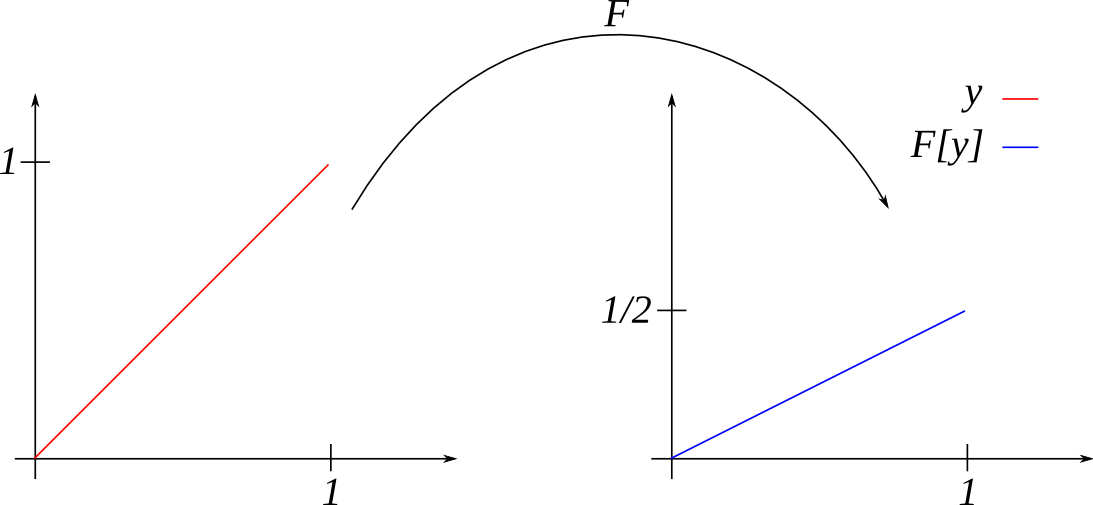
\includegraphics[width=0.45\textwidth]{images/07contraction1}
	} \hfill
	\subfloat[Decreasing sequence.]{
		\label{fig:07contraction2}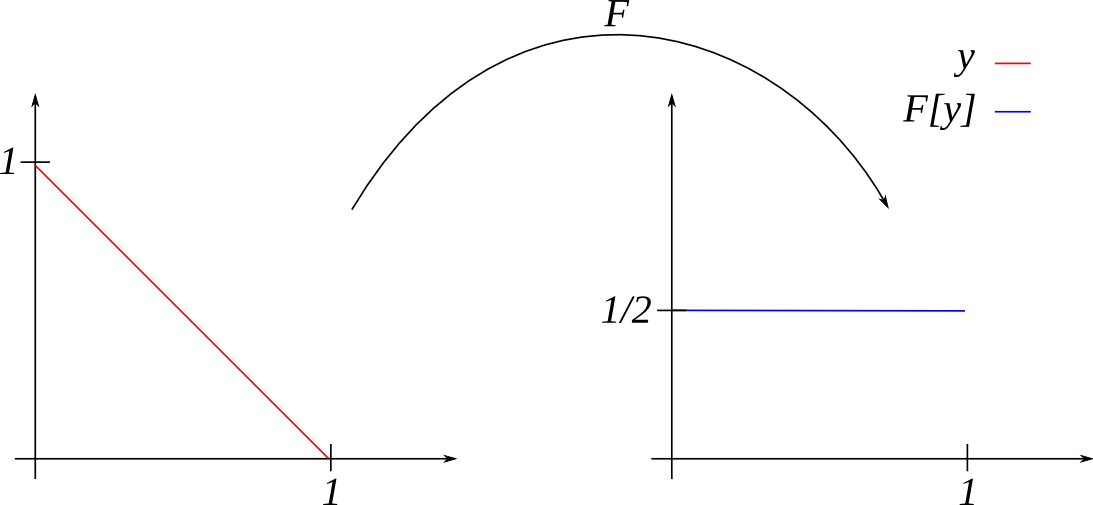
\includegraphics[width=0.45\textwidth]{images/07contraction2}
	}
	\caption{Example of the contraction operator $F$ acting on two sequences $y$.}
	\label{fig:07contraction}
\end{figure}

\subsection{Fixed Points}
Let $\vsp$ be a Banach space. Then $F:\mathbb{Y}\to\mathbb{Y}$ is a contraction with constant $K\in(0,1)$. Let $y_0\in\mathbb{Y}$. Given any $y_n$, let $y_{n+1}=F[y_n]$. We want to show that the sequence converges and that will give the solution, $y_{n+1}$.
$$||y_{n+2}-y_{n+1}|| = ||F[y_{n+1}]-F[y_n]|| \leq K||Y_{n+1}-y_n||$$
Suppose
$$||y_{n+k+1}-y_{n+k}||\leq K^k||y_{n+k}-y_n||$$
then
\begin{align}
\label{eq:converge}
||Y_{n+k+2}-y_{n+k+1}|| = ||F[y_{n+k+2}]-F[y_{n+k+1}]|| \leq K^{k+1}||y_{n+1}-y_n||
\end{align}
By induction (\ref{eq:converge}) holds for all $k\geq0$.

If we let $m\geq n$, then for $m=n+k+1$ we have
\begin{align*}
||y_m-y_n|| &\leq ||y_m-y_{m-1}|| + \cdots + ||y_{n+1}-y_n|| \\
&\leq \sum_{k=0}^{m-(n+1)} K^k||y_{n+1}-y_n|| \\
&\leq \sum_{k=0}^\infty K^k||y_{n+1}-y_n|| \\
&= \frac{1}{1-k}||y_{n+1}-y_n||
\end{align*}

If we let $n\geq N$, then we get
$$||y_m-y_n|| \leq \frac{K^n}{1-K}||y_1-y_0||\to0$$
This shows that $\{y_n\}$ is a Cauchy sequence. By compeleteness, there exists $\bar{y}\in\mathbb{Y}\text{ s.t. } y_n\to\bar{y}$. Then,
\begin{align*}
||\bar{y}-F[\bar{y}]|| &\leq ||\bar{y}-y_n|| - ||y_n-F[\bar{y}]|| \\
&= ||\bar{y}-y_n|| + ||F[y_{n-1}]-F[\bar{y}]|| \\
&\leq ||\bar{y}-y_n|| + K||y_{n-1}-\bar{y}||
\end{align*}
Both of the terms in the last inequaltiy go to zero, so
$$||\bar{y}-F[\bar{y}]|| = 0$$
and by the definition of a norm we get that $\bar{y}=F[\bar{y}]$. This means that $\bar{y}$ is a fixed point.

For uniqueness, suppose $\tilde{y}=F[\tilde{y}]$. Then,
\begin{align*}
||\bar{y}-\tilde{y}|| &= ||F[\bar{y}]-F[\tilde{y}]|| \\
&\leq K||\bar{y}-\tilde{y}|| \\
\therefore ||\bar{y}-\tilde{y}|| &= 0 \Rightarrow \tilde{y} = \bar{y}
\end{align*}

\begin{theorem}{Contraction Mapping Principle.}
This is also called the Banach Fixed Point Theorem. Let $\vsp$ be a Banach space and $F$ be a contraction, then there exists a unique solution to $y=F[y]$. Also, given $y_0\in\mathbb{Y}$ and letting $y_n\to y$ yields the solution.
\end{theorem}

As long as $F$ is a contraction and we pick the correct space to work in then we know the value iteration, $V=\mathcal{G}[V]$, will converge to a solution.


\end{document}

%%%%%%%%%%%%%%%%%%%%%%%%%%%%%%%%%%%%%%%%%%%%%%%%%%%%%%%%%%%%%